\documentclass[a4paper,11pt]{article}

\usepackage[english]{babel}
\usepackage{graphicx}
\usepackage{subfig}
\usepackage{xcolor}

\usepackage[
  pdftitle   = {Assignment}, 
  pdfauthor  = {Duke University},
  colorlinks = true,
  linkcolor  = blue,
  urlcolor   = blue,
  citecolor  = blue,
  bookmarks  = true,
  bookmarksopenlevel = 2]{hyperref}
\usepackage{amsmath,amssymb,amsthm,textcomp}
\usepackage{enumerate}
\usepackage{multicol}

\usepackage{geometry}
\geometry{total={210mm,297mm},
  left   = 28mm,
  right  = 28mm,
  top    = 30mm,
  bottom = 30mm,
  bindingoffset = 0mm 
}

%\linespread{1.3}
\newcommand{\linia}{\rule{\linewidth}{0.5pt}}

\usepackage{fancyhdr} 
\pagestyle{fancyplain}
\fancyhead{} 
\fancyfoot[C]{}
\fancyfoot[L]{\textit{Assignment: ICP}}
\fancyfoot[R]{\textit{\thepage}}
\renewcommand{\headrulewidth}{0.5pt}
\renewcommand{\footrulewidth}{0.5pt}
%\setlength{\headheight}{13.6pt} 

% Removes all indentation from paragraphs
\setlength\parindent{0pt}

% Horizontal rule command with 1 argument of height
\newcommand{\horrule}[1]{\rule{\linewidth}{#1}} 

\title{	
  \normalfont \normalsize 
  \textsc{
    Duke University \\ 
    Pratt School of Engineering \\
    Department of Electrical and Computer Engineering} \\ [25pt]
  \horrule{0.5pt} \\[0.4cm]
  \huge Assignment: Iterative Closest Point (ICP) \\
  \horrule{2pt} \\[0.5cm]  
}
\author{Oscar Ramos (oscar.ramos\@ duke.edu)\\
Kris Hauser(kris.hauser\@ duke.edu) }
\date{\normalsize\today}   



\begin{document}
\maketitle
\thispagestyle{empty}



\section{Background}

The Iterative Closest Point is an algorithm used to minimize the difference
between two objects related by a rigid-body transformation, with the objective
of recovering the most likely transformation. Given lists of corresponding points on 
each object:
\begin{align*}
  S_1 & = \{ p_1, p_2, \cdots, p_n \} \\
  S_2 & = \{ r_1, r_2, \cdots, r_n \}
\end{align*}
where $p_i,r_i \in \mathbb{R}^k$, the objective is to find a translation
$t \in \mathbb{R}^k$ and rotation $R \in SO(k)$ that solve the problem 
\begin{equation}
  \label{eq:general_minimization}
  \min_{R,t} \sum_{i} d(p_i, Rr_i+t)
\end{equation}
where $k=2$ or $3$, and $d(\cdot,\cdot)$ is a distance such as the Euclidean distance and $SO(k)$ is the
group of rotation matrices in $\mathbb{R}^k$. 

An important first step is to estimate the corresponding pairs $S_1$ and $S_2$. Typical
matching approaches include exhaustive closest point matching, projections,
space partitioning ($k$-d trees), amongst others.  A variety of outlier rejection
techniques may be used here as well.  The ICP algorithm alternates the two steps of
correspondence detection and error minimization until some notion of convergence is
reached.

In this assignment we will start
with a very simple 2D case and then we will address the problem for the 3D case.


\section{ICP in 2D}

In this part, we will focus on implementing the ICP algorithm for the planar
case using two simple images.  You should place all your work in the file
\texttt{triangles\_2d.py}.

Each image contains the same triangle but with a
different position and orientation as shown in Fig.~\ref{fig:triangles}.
\begin{figure} [ht]
  \centering \footnotesize
  \subfloat [First triangle]
  { 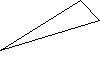
\includegraphics[width=0.17\linewidth]{images/image_1} 
  } \hspace{2cm}
  \subfloat [Second triangle]
  { 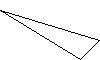
\includegraphics[width=0.17\linewidth]{images/image_2}
  }
  \caption{Two triangles in 2D}
  \label{fig:triangles}
\end{figure}
Recall that in 2D, a translation is described by a position vector
$t=(x_{t},y_{t}) \in \mathbb{R}^2$, and a rotation by a matrix $R \in SO(2)$
with components
\begin{equation*}
  R = \begin{bmatrix} 
    \cos(\theta) & -\sin(\theta) \\ 
    \sin(\theta) & \cos(\theta)
\end{bmatrix}
\end{equation*}
where $\theta$ is the angle of rotation. The objective is to find the
translation $t$ and the rotation $R$ of the second triangle with respect to the
first triangle.


\subsection{Preprocessing} 

To load images using Python, the Python Imaging Library (PIL) needs to be used.
and it can be installed from the developer website (http://www.pythonware.com/products/pil/)).

The images of the triangles
to be used in this part can be found in the folder \texttt{data/2d}.  Note that,
like in real images,
there is some noise around the triangles.  Before starting ICP, it is a good
idea to remove that noise.  The script will load the files and extract only those
points whose values are less than 128 (darker than 50\% grey).

\subsection{Finding correspondences} 

In this exercise we are dealing with a small image and there are not many points
(less than 200 points) that constitute the triangles. Therefore, we can apply an
exhaustive search to find the closest points. (However, note that this approach
is not acceptable in cases where there are many points such as for the 3D point
clouds in the next section.)

{\bf Task 1.}   Using the square of the Euclidean distance 
\begin{equation*}
d(p_i,r_i) = \Vert p_i - r_i \Vert^2
\end{equation*}
to measure how close the points $p_i$ and $r_i$ are, find the matching pairs
for the two triangles using an exhaustive search. In other terms, for every
point in triangle 1, find the closest point in triangle 2.  Your code for this
question should go in \texttt{get\_closest\_points\_2d()}.

Usually the result from finding the closest points contains some (or many)
outliers which need to be rejected since otherwise they would contaminate the
data when computing the following steps. Thus, it is a good idea to apply a
threshold on the matching points based on how close they are (using the chosen
distance measure). This can be done after finding the closest points or it can
be done at the moment of finding them.

{\bf Task 2.}  Implement an outlier rejection criterion in \texttt{threshold\_closest\_points()}
that discards the candidate pairs with distance exceeding some threshold.   Later you will
play around with the \texttt{threshold} value in \texttt{get\_correspondences()} to make
your algorithm more robust.


\subsection{Minimizing the error}

After the matching pairs between the two sets (triangles) has been found, the
next step is to find the rotation $R$ and translation $t$ that minimizes the
error function. In this case, using the Euclidean distance as the error function,
\eqref{eq:general_minimization} will be written as
\begin{equation}
  \label{eq:1}
  \min_{R,t} \sum_{i=1}^N \Vert p_i - (Rr_i + t) \Vert^2
\end{equation}
where $p_i$ and $r_i$ are the corresponding points in the first and second
triangles, respectively, and we assume that there are $N$ correspondences.

{\bf Task 3.}   Implement a method that minimizes \eqref{eq:1} in \texttt{icp\_step()}.
This minimization problem can be solved in different ways. One of them is using an SVD
decomposition \cite{Arun87}.   You are suggested to use the SVD solution,
since it is relatively straightforward. However, if you prefer, you can
implement any other method that solves \eqref{eq:general_minimization}, such
as gradient descent.

To implement the SVD method, first the centroids for both triangles need to be computed. They are given by
\begin{equation*}
  \mu_p = \frac{1}{N}\sum_{i=1}^{N} p_i \qquad \qquad \mu_r =
  \frac{1}{N}\sum_{i=1}^{N} r_i
\end{equation*}
and then these centroids can be subtracted from the initial points
\begin{equation*}
  \tilde{p}_i = p_i - \mu_p \qquad \qquad \tilde{r}_i = r_i - \mu_r.
\end{equation*}
It can be shown \cite{Arun87} that using the previous operations and replacing
into the original problem, the minimization problem
\eqref{eq:general_minimization} is reduced to
\begin{equation}
  \label{eq:min_rotation}
  \min_{R} \sum_{i=1}^N \Vert \tilde{p}_i - R\tilde{r}_i \Vert^2.
\end{equation}
The covariance matrix of the points corresponding to both triangles can be
computed as
\begin{equation*}
  H = \sum_{i=1}^{N} \tilde{p}_i\tilde{r}_i^T = 
  \begin{bmatrix}
    \sum_{i=1}^{N} \tilde{p}_{ix}\tilde{r}_{ix} &
    \sum_{i=1}^{N} \tilde{p}_{ix}\tilde{r}_{iy} \\
    \sum_{i=1}^{N} \tilde{p}_{iy}\tilde{r}_{ix} &
    \sum_{i=1}^{N} \tilde{p}_{iy}\tilde{r}_{iy} 
  \end{bmatrix}
\end{equation*}
where the components of the 2D points are
$\tilde{p}_i = (\tilde{p}_{ix}, \tilde{p}_{iy})$ and
$\tilde{r}_i = (\tilde{r}_{ix}, \tilde{r}_{iy})$. Using an Singular Value
Decomposition (SVD), the covariance matrix $H$ can be rewritten as
\begin{equation*}
  H = U \Sigma V^T
\end{equation*}
where $U$ and $V$ are orthogonal matrices and $\Sigma$ is a diagonal matrix
containing the singular values of $H$ in its diagonal. It can be shown
\cite{Arun87} that using the SVD decomposition of the covariance matrix, the
solution to \eqref{eq:min_rotation} is given by
\begin{equation}
  \label{eq:4}
  R = UV^T \qquad  \text{and} \qquad    t = \mu_p - R \mu_r.
\end{equation}
Actually, there is another potential solution that is a critical point of the
minimization, which is $R=VU^T$.  One of these is a minimum and the other is a
maximum.  Your algorithm should test for which one is a minimizer.
To solve the SVD you should use the numpy.linalg.svd(H) method from the numpy
package (the scipy package is acceptable as well). Numpy is
included in most Python distributions.  You can put your code for this in
\texttt{compute\_error\_minimizing\_rotation()}.

{\bf Task 4.}  Debug your ICP algorithm and play with the initial conditions and
the thresholding parameter.  What is the best value for the parameter?
Why do you think this is the case?

Note: if you have the matplotlib Python package installed, the triangles and their
correspondences at each stage of the ICP will be displayed to you.  This should
be quite helpful for debugging.


\section{ICP for a 3D point cloud}

In this part of the assignment we will extend the usage of ICP to the 3D case. 
For the amazon picking challenge, several point clouds have been acquired for
different objects and they are available at
\texttt{http://rll.berkeley.edu/amazon\_picking\_challenge}. The point clouds
that we will be using originally come from that database, but their format has
been modified to be easily read in Python.

\subsection{Matching with a Known Object}

The first question will ask you to implement ICP for 3D point clouds.
The models of some selected objects in the APC can be
found in \texttt{data/models} and are in json format. The depth maps to be used
in this part can be found in \texttt{data/processed\_depth}, also in json
format. To read these files, use the script called
\texttt{match\_3d.py} which will read the \texttt{school\_glue} file by
default. OpenGL will show the model in its reconstructed colors, the depth map in blue, and an axis
at the coordinates origin (red, green and blue represent the $x$, $y$ and $z$
axis, respectively).  For testing, you should use any of the four depth maps in \texttt{data/processed\_depth}.

{\bf Task 5.}  Implement the \texttt{icp()} function in \texttt{match\_3d.py}.
The steps to follow for the implementation are similar to the 2D
case. However, there are several issues you must address when scaling up to 3D.

First, there are many points in the depth map and an exhaustive search
is not a practical approach (you can try, but it will take a lot of time). One
of the simplest approaches to addressing this challenge is to sample the data (both
data sets) uniformly or randomly before attempting to match the points. Another
approach can be to use a faster point location data structure, such as a grid or
a K-d tree.

Also, note that there are some points in the depth map that are very close to
each other within some small margin. It can be useful to only keep one of those
points before doing the pair matching in order to have fewer possible
pairs. Another problem that might occur is that some points can be too close to
the model and can generate a considerable bias. In this case, you might enforce
a limit on the number of points that may be matched to a single point.

The translation and rotation matching portion of this task is very similar to that
of the 2D case.  If the SVD method is used, note that the covariance matrix $H$ from the 2D case
needs to be modified for the 3D points as
\begin{equation*}
  H = \sum_{i=1}^{N} \tilde{p}_i\tilde{r}_i^T = 
  \begin{bmatrix}
    \sum_{i=1}^{N} \tilde{p}_{ix}\tilde{r}_{ix} &
    \sum_{i=1}^{N} \tilde{p}_{ix}\tilde{r}_{iy} &
    \sum_{i=1}^{N} \tilde{p}_{ix}\tilde{r}_{iz} \\
    \sum_{i=1}^{N} \tilde{p}_{iy}\tilde{r}_{ix} &
    \sum_{i=1}^{N} \tilde{p}_{iy}\tilde{r}_{iy} &
    \sum_{i=1}^{N} \tilde{p}_{iy}\tilde{r}_{iz} \\
    \sum_{i=1}^{N} \tilde{p}_{iz}\tilde{r}_{ix} &
    \sum_{i=1}^{N} \tilde{p}_{iz}\tilde{r}_{iy} &
    \sum_{i=1}^{N} \tilde{p}_{iz}\tilde{r}_{iz} 
  \end{bmatrix}
\end{equation*}
but the general procedure remains similar. 


\subsection{Matching unknown objects}

Your final task will be to use ICP to attempt to discover which object
is present in an ``unknown'' scene.  The \texttt{detect\_3d.py} file will
run your ICP algorithm from Task 5 on all four known objects to match them
to a given scene.  You will also implement a scoring function that will
assess the matching error for a given ICP solution.  This function should
help you distinguish between objects in a given scene.

As an error function you may wish to simply return the sum of squared distances in the
ICP correspondences, or do something different to achieve better performance.

{\bf Task 6.}  Implement a \texttt{matching\_error(object,scene)} function in \texttt{detect\_3d.py} that (hopefully) gives lower errors to objects that are matched well to a given scene.   Investigate its performance empirically in detecting the correct object on the four scenes (you will do this by changing the \texttt{scene} variable).  Report your results in the
commented-out area provided for you.


\begin{thebibliography}{9}

\bibitem{Arun87}
  Arun, K.S., Huang, T.S. and Blostein S.D.,
  Least-squares fitting of two 3-D point sets, 
  \emph{IEEE Transactions on Pattern Analysis and Machine Intelligence}.
  9(5): 698-700,
  1987.
\end{thebibliography}


\end{document}
